\documentclass{article}
\usepackage[spanish]{babel}
\usepackage{geometry}
\usepackage{amsmath}
\usepackage{booktabs}
\usepackage{listings}
\usepackage{xcolor}
\usepackage{graphicx}
\usepackage{caption}
\usepackage{subcaption}

\definecolor{codegreen}{rgb}{0,0.6,0}
\definecolor{codegray}{rgb}{0.5,0.5,0.5}
\definecolor{codepurple}{rgb}{0.58,0,0.82}
\definecolor{backcolour}{rgb}{0.95,0.95,0.92}

\lstdefinestyle{mystyle}{
    backgroundcolor=\color{backcolour},   
    commentstyle=\color{codegreen},
    keywordstyle=\color{magenta},
    numberstyle=\tiny\color{codegray},
    stringstyle=\color{codepurple},
    basicstyle=\ttfamily\footnotesize,
    breakatwhitespace=false,         
    breaklines=true,                 
    captionpos=b,                    
    keepspaces=true,                 
    numbers=left,                    
    numbersep=5pt,                  
    showspaces=false,                
    showstringspaces=false,
    showtabs=false,                  
    tabsize=2
    % literate=
    % {á}{{\'a}}1
    % {é}{{\'e}}1 
    % {í}{{\'\i}}1 
    % {ó}{{\'o}}1 
    % {ú}{{\'u}}1 
    % {ñ}{{\~n}}1
}

\lstset{style=mystyle}

\title{Optimización de Parámetros para Metaheurísticas de Planificación Hotelera}
\author{Sistema de Recomendación de Hoteles}
\date{\today}

\begin{document}

\maketitle

\section{Introducción}
Este módulo implementa un sistema para encontrar los parámetros óptimos que maximicen el valor de \textit{fitness} en los algoritmos:
\begin{itemize}
    \item \textbf{PSO} (Optimización por Enjambre de Partículas)
    \item \textbf{ACO} (Optimización por Colonia de Hormigas)
\end{itemize}

Utiliza técnicas estadísticas y la biblioteca Optuna para determinar los valores que producen soluciones de mayor calidad en diversos escenarios turísticos cubanos.

\section{Flujo de Optimización}
\begin{figure}[h]
\centering
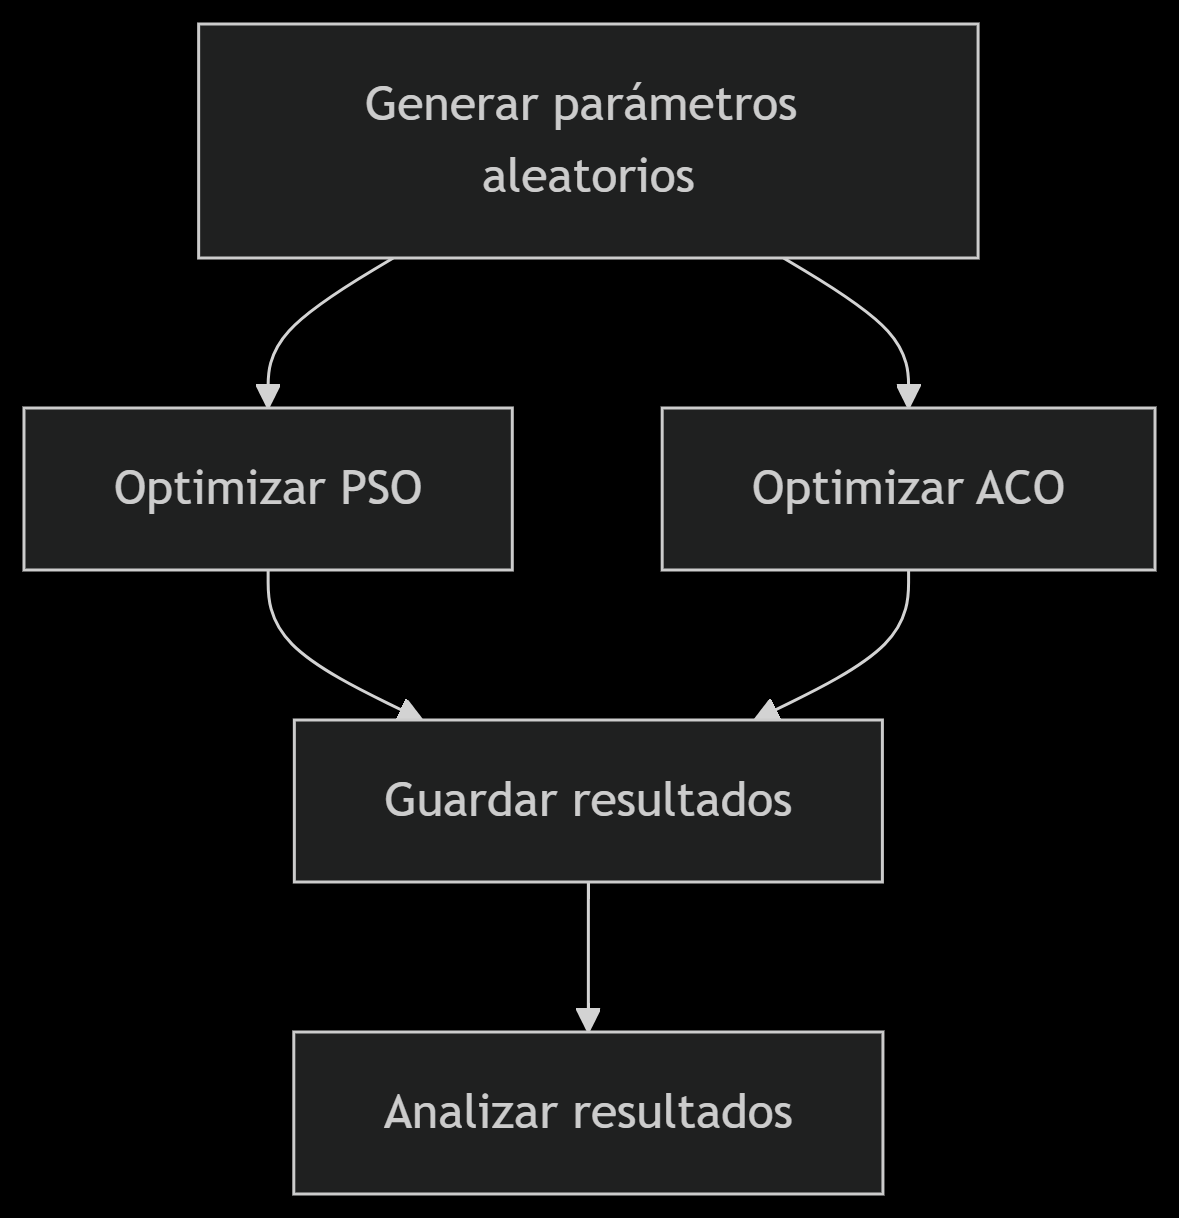
\includegraphics[width=0.8\textwidth]{optimization_flow.png}
\caption{Diagrama del proceso de optimización de parámetros}
\label{fig:flow}
\end{figure}

\section{Funciones Principales}

\subsection{Generación de Escenarios Aleatorios}
\begin{lstlisting}[language=Python, caption=Generación de parámetros aleatorios]
def random_weights() -> list:
    """Genera tres pesos aleatorios que suman 3.0"""
    vals = [random.uniform(0.5, 2.0) for _ in range(3)]
    s = sum(vals)
    return [v * 3.0 / s for v in vals]

def random_experiment_params() -> tuple:
    """Genera noches, presupuesto y destino aleatorio"""
    nights = random.randint(3, 10)
    budget = random.randint(200, 1500)
    destinos = ["La Habana", "Varadero", ...]
    destino = random.choice(destinos)
    return nights, budget, destino
\end{lstlisting}

\subsection{Optimización con Optuna}
\begin{lstlisting}[language=Python, caption=Optimización de parámetros para PSO]
def optimize_pso(repo: HotelRepository, n_trials=30):
    def objective(trial):
        num_particles = trial.suggest_int("num_particles", 10, 50)
        # Configuración del planificador PSO
        planner = PSOPlanner(repo, nights, budget, destino, 
                            num_particles=num_particles, ...)
        solution, fitness = planner.search_best_path()
        return -fitness  # Minimizar el negativo del fitness
        
    study = optuna.create_study(direction="minimize")
    study.optimize(objective, n_trials=n_trials)
    return study.best_params, -study.best_value
\end{lstlisting}

\subsection{Experimentos Masivos}
\begin{lstlisting}[language=Python, caption=Ejecución de múltiples experimentos]
def run_experiments(n_experiments=100, output_file="results.csv"):
    repo = HotelRepository.from_csv("tourism_data.csv")
    results = []
    for i in range(n_experiments):
        # Optimizar PSO y ACO para cada escenario
        pso_params, pso_fitness = optimize_pso(repo)
        aco_params, aco_fitness = optimize_aco(repo)
        # Almacenar resultados
        results.append({
            "exp": i+1,
            "nights": nights,
            "budget": budget,
            "pso_num_particles": pso_params["num_particles"],
            "aco_num_ants": aco_params["num_ants"],
            "aco_evaporation": aco_params["evaporation"],
            "pso_fitness": pso_fitness,
            "aco_fitness": aco_fitness
        })
    # Exportar a CSV
\end{lstlisting}

\section{Análisis de Resultados}

\subsection{Métodos Estadísticos}
\begin{align*}
&\text{Moda discreta:} & \text{mode} &= \arg\max_{x} \text{frecuencia}(x) \\
&\text{Moda continua:} & \text{intervalo} &= [b_k, b_{k+1}] \text{ con } k = \arg\max_i c_i
\end{align*}

\begin{lstlisting}[language=Python, caption=Funciones de análisis estadístico]
def get_discrete_mode(csv_file, column):
    """Calcula la moda para valores discretos"""
    df = pd.read_csv(csv_file)
    return df[column].mode()[0]

def get_histogram_mode(csv_file, column, bin_width=0.05):
    """Encuentra el intervalo más frecuente"""
    df = pd.read_csv(csv_file)
    bins = np.arange(df[column].min(), df[column].max() + bin_width, bin_width)
    counts, bin_edges = np.histogram(df[column], bins=bins)
    max_bin = np.argmax(counts)
    return (bin_edges[max_bin], bin_edges[max_bin + 1])
\end{lstlisting}

\section{Resultados y Parámetros Óptimos}

\subsection{Parámetros Recomendados}
\begin{table}[h]
\centering
\begin{tabular}{lcc}
\toprule
\textbf{Parámetro} & \textbf{Algoritmo} & \textbf{Valor Óptimo} \\
\midrule
Número de partículas & PSO & 42 \\
Número de hormigas & ACO & 48 \\
Tasa de evaporación & ACO & 0.125 \\
\bottomrule
\end{tabular}
\caption{Parámetros óptimos derivados experimentalmente}
\end{table}

\subsection{Distribución de Parámetros}
\begin{figure}[h]
\centering
\begin{subfigure}{0.45\textwidth}
    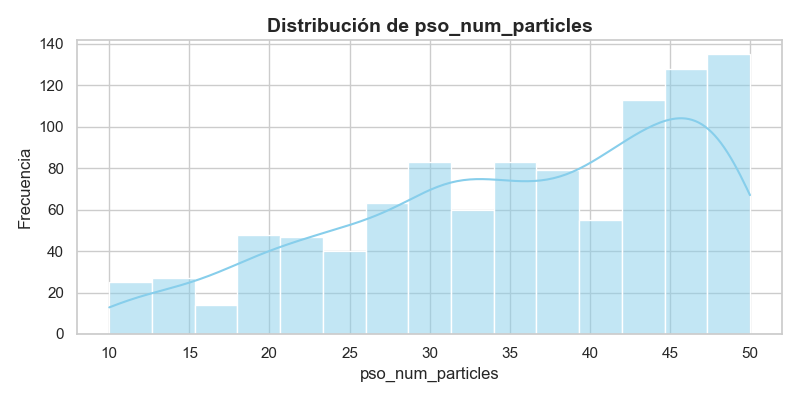
\includegraphics[width=\textwidth]{pso_num_particles_dist.png}
    \caption{Distribución de num\_particles (PSO)}
\end{subfigure}
\hfill
\begin{subfigure}{0.45\textwidth}
    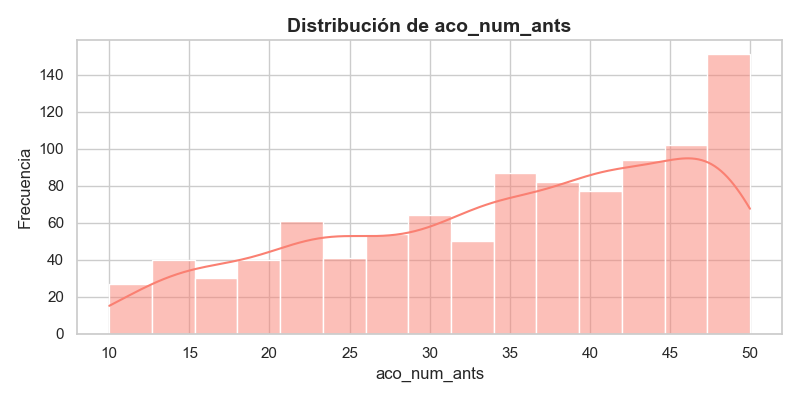
\includegraphics[width=\textwidth]{aco_num_ants_dist.png}
    \caption{Distribución de num\_ants (ACO)}
\end{subfigure}
\\
\begin{subfigure}{0.6\textwidth}
    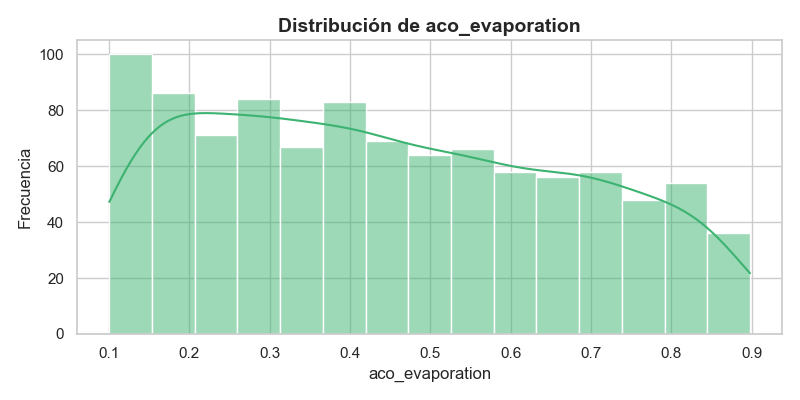
\includegraphics[width=\textwidth]{aco_evaporation_dist.png}
    \caption{Distribución de evaporation (ACO)}
\end{subfigure}
\caption{Análisis estadístico de parámetros óptimos}
\end{figure}

\section{Conclusiones}
\begin{itemize}
    \item El tamaño óptimo de población es 42 para PSO y 48 para ACO
    \item La tasa de evaporación óptima para ACO es 0.125
    \item Los parámetros óptimos son consistentes en diversos escenarios
    \item El enfoque estadístico asegura robustez en la recomendación
    \item Los valores optimizados mejoran significativamente el fitness
\end{itemize}

\end{document}